\documentclass{summarysheet}

\begin{document}

\maketitle{6}{Dynamics of Circular Motion}


\begin{multicols}{2}

\begin{topicbox}{The $rtz$ Coordinate System}

\noindent An $x$-$y$-$z$ coordinate system is not great for dealing with circular motion.  Better is the $r$-$t$-$z$ coordinate system, where:
\begin{itemize}
\item the origin is at the particle's position,
\item the $r$ (radial) axis points from the particle to the centre of the circle,
\item the $t$ (tangential) axis points tangent to the circle in the counterclockwise direction, and
\item the $z$ axis is perpendicular to the plane of motion.
\end{itemize}

\begin{center}
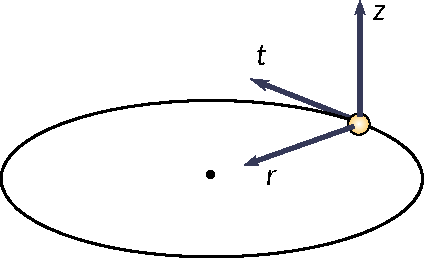
\includegraphics[scale=0.6]{fig_rtz.pdf}
\end{center}

\end{topicbox}

\begin{topicbox}{Newton's Second Law for Circular Motion}

\noindent Recall that for circular motion the acceleration has a radial ($r$) component related to the change in direction and a tangential ($t$) component related to the chnage in speed.  In the $rtz$ coordinate system, then, Newton's second law take the form

\begin{multicols}{2}


\begin{teqbox}
\begin{align*}
F_\text{net $r$} & = ma_r  = \frac{mv^2}{r} = m\omega^2 r \\
F_\text{net $t$} & = ma_t  = m \alpha r \\
F_\text{net $z$} & = ma_z = 0 \\
\end{align*}
\end{teqbox}

\begin{center}
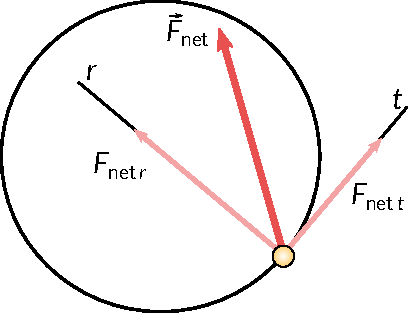
\includegraphics[scale=0.6]{fig_fnet.pdf}
\end{center}

\end{multicols}

\end{topicbox}


\begin{topicbox}{MODEL: Uniform Circular Motion}

\noindent For \emph{uniform circular motion}, $a_t = 0$, so Newton's second law is
\begin{teqbox}
\begin{align*}
F_\text{net $r$} & = \frac{mv^2}{r} = m\omega^2 r \\
F_\text{net $t$} & = 0\\
F_\text{net $z$} & = 0 \\
\end{align*}
\end{teqbox}

\end{topicbox}

\begin{topicbox}{MODEL: Constant Angular Acceleration}

\noindent For \emph{nonuniform circular motion}, Newton's second law is
\begin{teqbox}
\begin{align*}
F_\text{net $r$} & = m\omega^2 r \\
F_\text{net $t$} & = m\alpha r\\
F_\text{net $z$} & = 0 \\
\end{align*}
\end{teqbox}

\end{topicbox}

\begin{topicbox}{APPLICATION: Circular Orbits}

\noindent In a circular orbit, the only force acting on the object (for example, the International Space Station or a satellite) is \emph{gravity}.  But we can't use the \emph{flat Earth approximation} for this; instead, we model gravity as
\begin{eqbox}
\vec{F}_\text{G} = (mg, \text{toward centre}).
\end{eqbox}

Since this force is \emph{radial} (or \emph{central}), the orbit is uniform circular motion with acceleration $g$:
\[
a_r = \frac{v_\text{orbit}^2}{r} = g.
\]
The speed of the orbiting object is then
\begin{eqbox}
v_\text{orbit} = \sqrt{gr}.
\end{eqbox}

\begin{center}
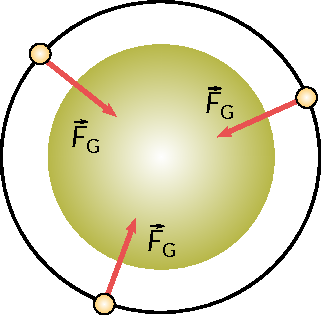
\includegraphics[scale=0.6]{fig_orbit.pdf}
\end{center}

\end{topicbox}

\begin{topicbox}{APPLICATION: Roller Coasters}

\noindent A roller coaster doing a loop-the-loop is in \emph{nonuniform circular motion} -- it slows down on its way up and speeds up on its way down.  But at the top and bottom of the loop, the cart has only \emph{radial} forces.  

\begin{multicols}{2}

At the bottom, Newton's second law says
\[
F_\text{net $r$} = n - mg = \frac{mv^2}{r},
\]
or
\[
n = mg + \frac{mv^2}{r},
\]
so you feel heavier than normal.

At the top, we have 
\[
F_\text{net $r$} = n + mg = \frac{mv^2}{r},
\]
or
\[
n = \frac{mv^2}{r} - mg.
\]


\begin{center}
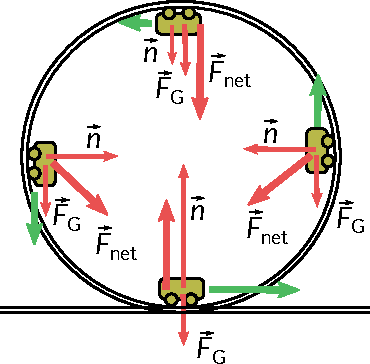
\includegraphics[scale=0.65]{fig_rc.pdf}
\end{center}
\end{multicols}

When the normal force goes to \emph{zero} -- meaning the cart loses contact with the track -- the cart will no longer be in circular motion.  This occurs at a \emph{critical speed}
\begin{eqbox}
v_c = \sqrt{gr}.
\end{eqbox}
Any speed \emph{less} than this and the cart won't complete the loop.

\end{topicbox}


\end{multicols}



\makebanner{Mechanics}

\end{document}



